\documentclass[12pt]{amsart}
\usepackage[T1]{fontenc}
\usepackage[utf8]{inputenc}

\usepackage[top=1.95cm, bottom=1.95cm, left=2.35cm, right=2.35cm]{geometry}

\usepackage{hyperref}
\usepackage{enumitem}
\usepackage{tcolorbox}
\usepackage{float}
\usepackage{cleveref}
\usepackage{multicol}
\usepackage{fancyvrb}
\usepackage{amsmath}
\usepackage[french]{babel}
\usepackage[
    type={CC},
    modifier={by-nc-sa},
    version={4.0},
]{doclicense}

\newcommand\floor[1]{\left\lfloor #1 \right\rfloor}

\usepackage{tnsmath}


\newtheorem{fact}{Fait}[section]
\newtheorem{example}{Exemple}[section]
\newtheorem{remark}{Remarque}[section]
\newtheorem*{proof*}{Preuve}

\setlength\parindent{0pt}

\floatstyle{boxed}
\restylefloat{figure}


\DeclareMathOperator{\taille}{\text{\normalfont\texttt{taille}}}

\newcommand\sqseq[2]{\fbox{$#1$}_{\,\,#2}}


\DefineVerbatimEnvironment{rawcode}%
    {Verbatim}%
    {tabsize=4,%
     frame=lines, framerule=0.3mm, framesep=2.5mm}



\begin{document}

\title{BROUILLON - Sommer les carrés des chiffres d'un naturel}
\author{Christophe BAL}
\date{6 Juin 2018 -- 28 Mars 2019}

\maketitle

\begin{center}
    \itshape
    Document, avec son source \LaTeX, disponible sur la page

    \url{https://github.com/bc-writings/bc-public-docs/tree/main/drafts}.
\end{center}


\bigskip


\begin{center}
    \hrule\vspace{.3em}
    {
        \fontsize{1.35em}{1em}\selectfont
        \textbf{Mentions \og légales \fg}
    }

    \vspace{0.45em}
    \doclicenseThis
    \hrule
\end{center}


\bigskip
\setcounter{tocdepth}{1}
\tableofcontents



\section{Faire une tête au carré à tous les entiers naturels}

Dans un repère orthogonal, donnons nous la parabole $\setgeo{P} : y = x^2$ . Plaçons-y les points $A$ , $B$ et $S$ d'abscisses respectives $a$ , $b$ et  $s = a + b$ .
Observez
\footnote{
	Le lieu de téléchargement de ce document contient un fichier GeoGebra \texttt{base-tool.ggb} manipulable dynamiquement pour vérifier combien il est aisé de conjecturer quelque chose.
}
les trois cas ci-dessous et essayez de conjecturer quelque chose \emph{(la réponse est donnée dans la page suivante)}
\footnote{
	On peut géométriquement additionner modulo $2 \pi$ sur un cercle.
	Or $x^2 - y^2$ et $x^2 - y$ sont des formes quadratiques avec des propriétés géométriques communes.
	C'est là l'origine de la recherche proposée ici.
}.


\vspace{2.5em}

\begin{multicols}{2}
	\center
	\footnotesize
	\itshape
	
	\fbox{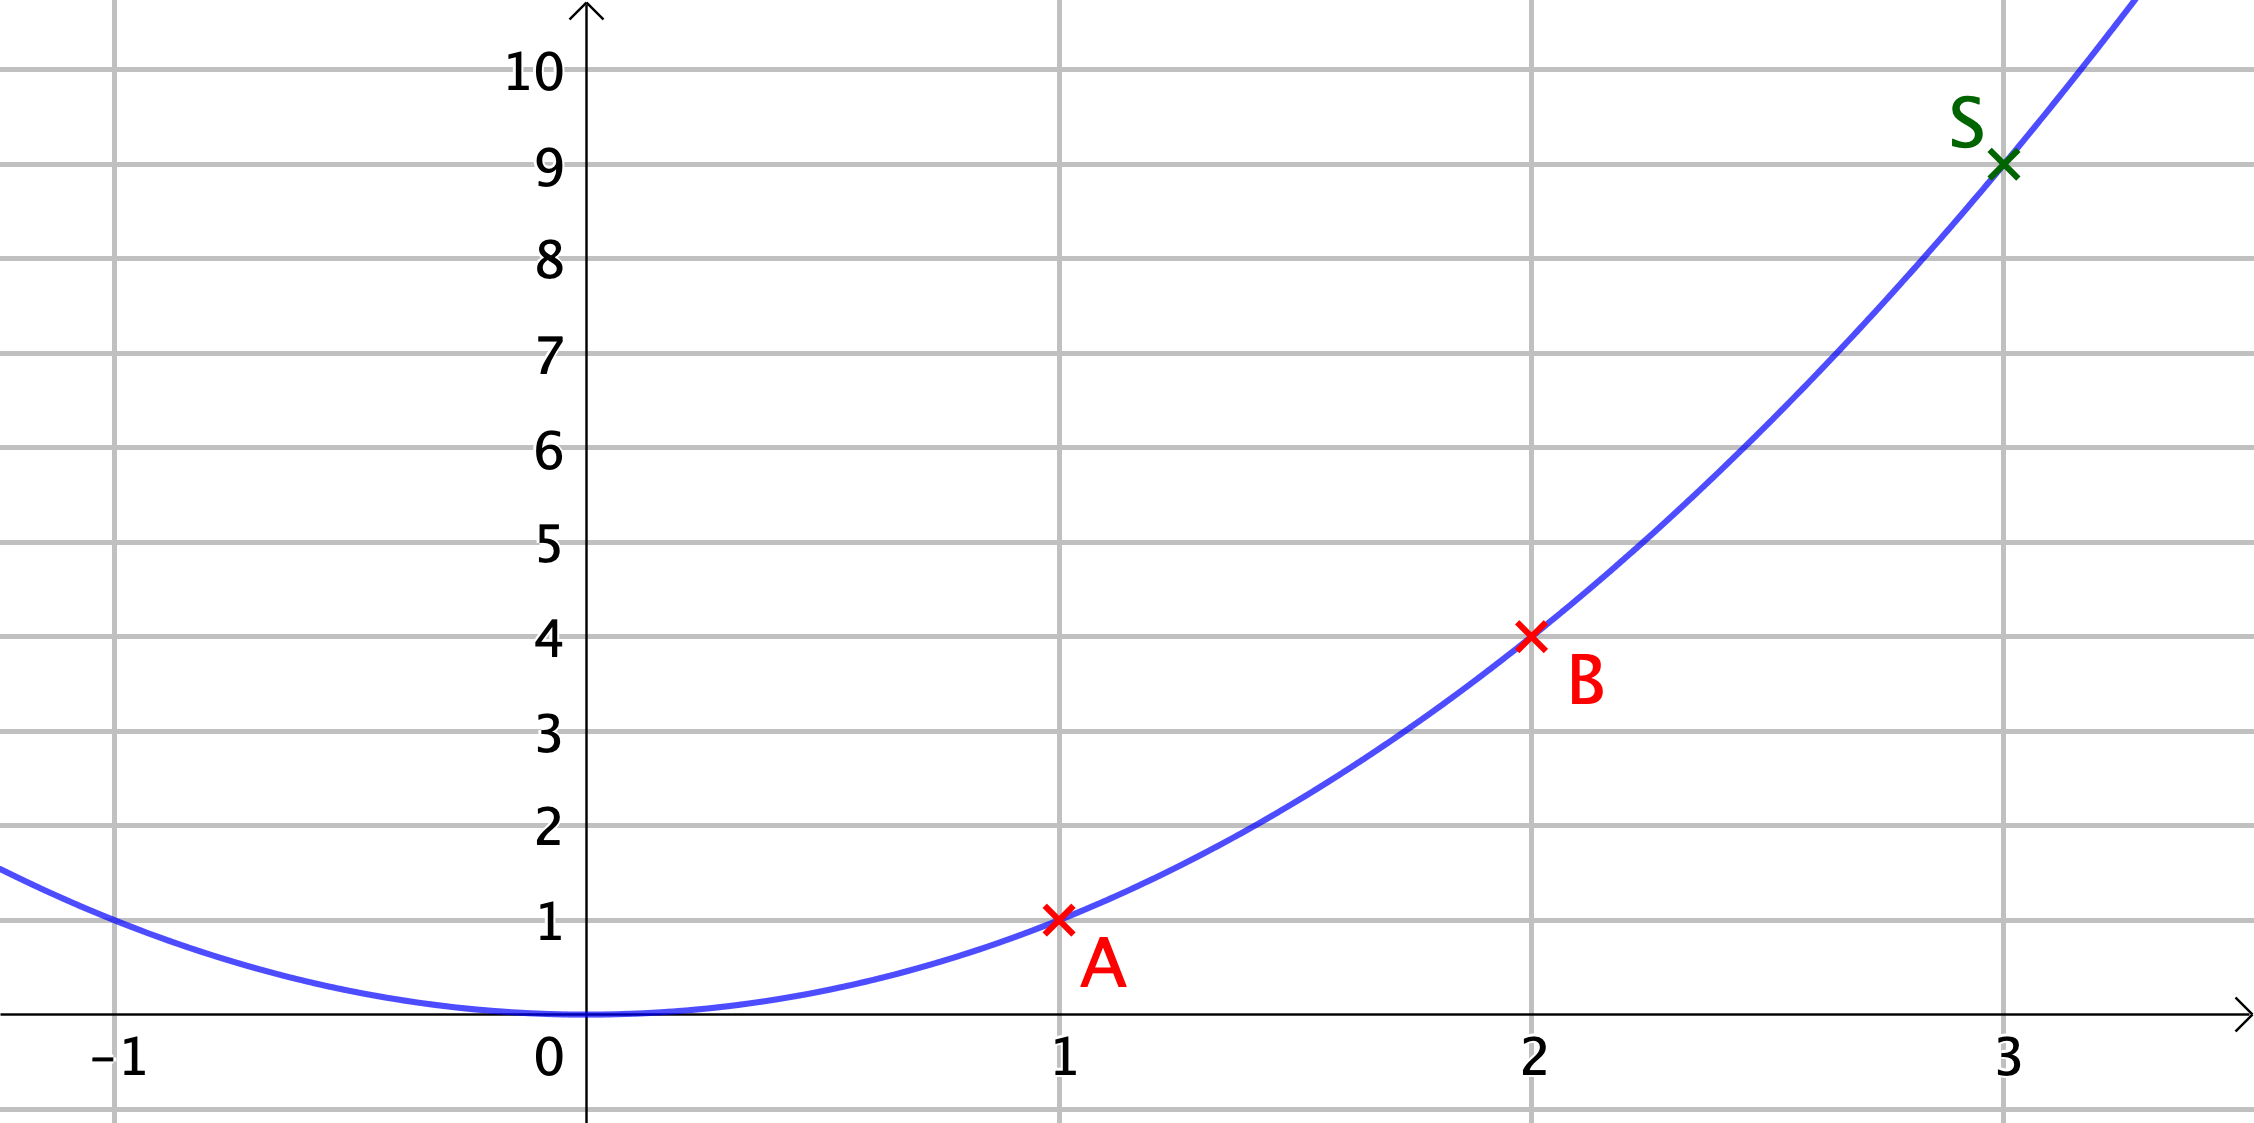
\includegraphics[scale = .8]{addition-on-parabolas/conjecture/a-and-b-positive.png}}
	
	\smallskip
	Cas où $a > 0$ et $b > 0$

	\columnbreak
	
	\fbox{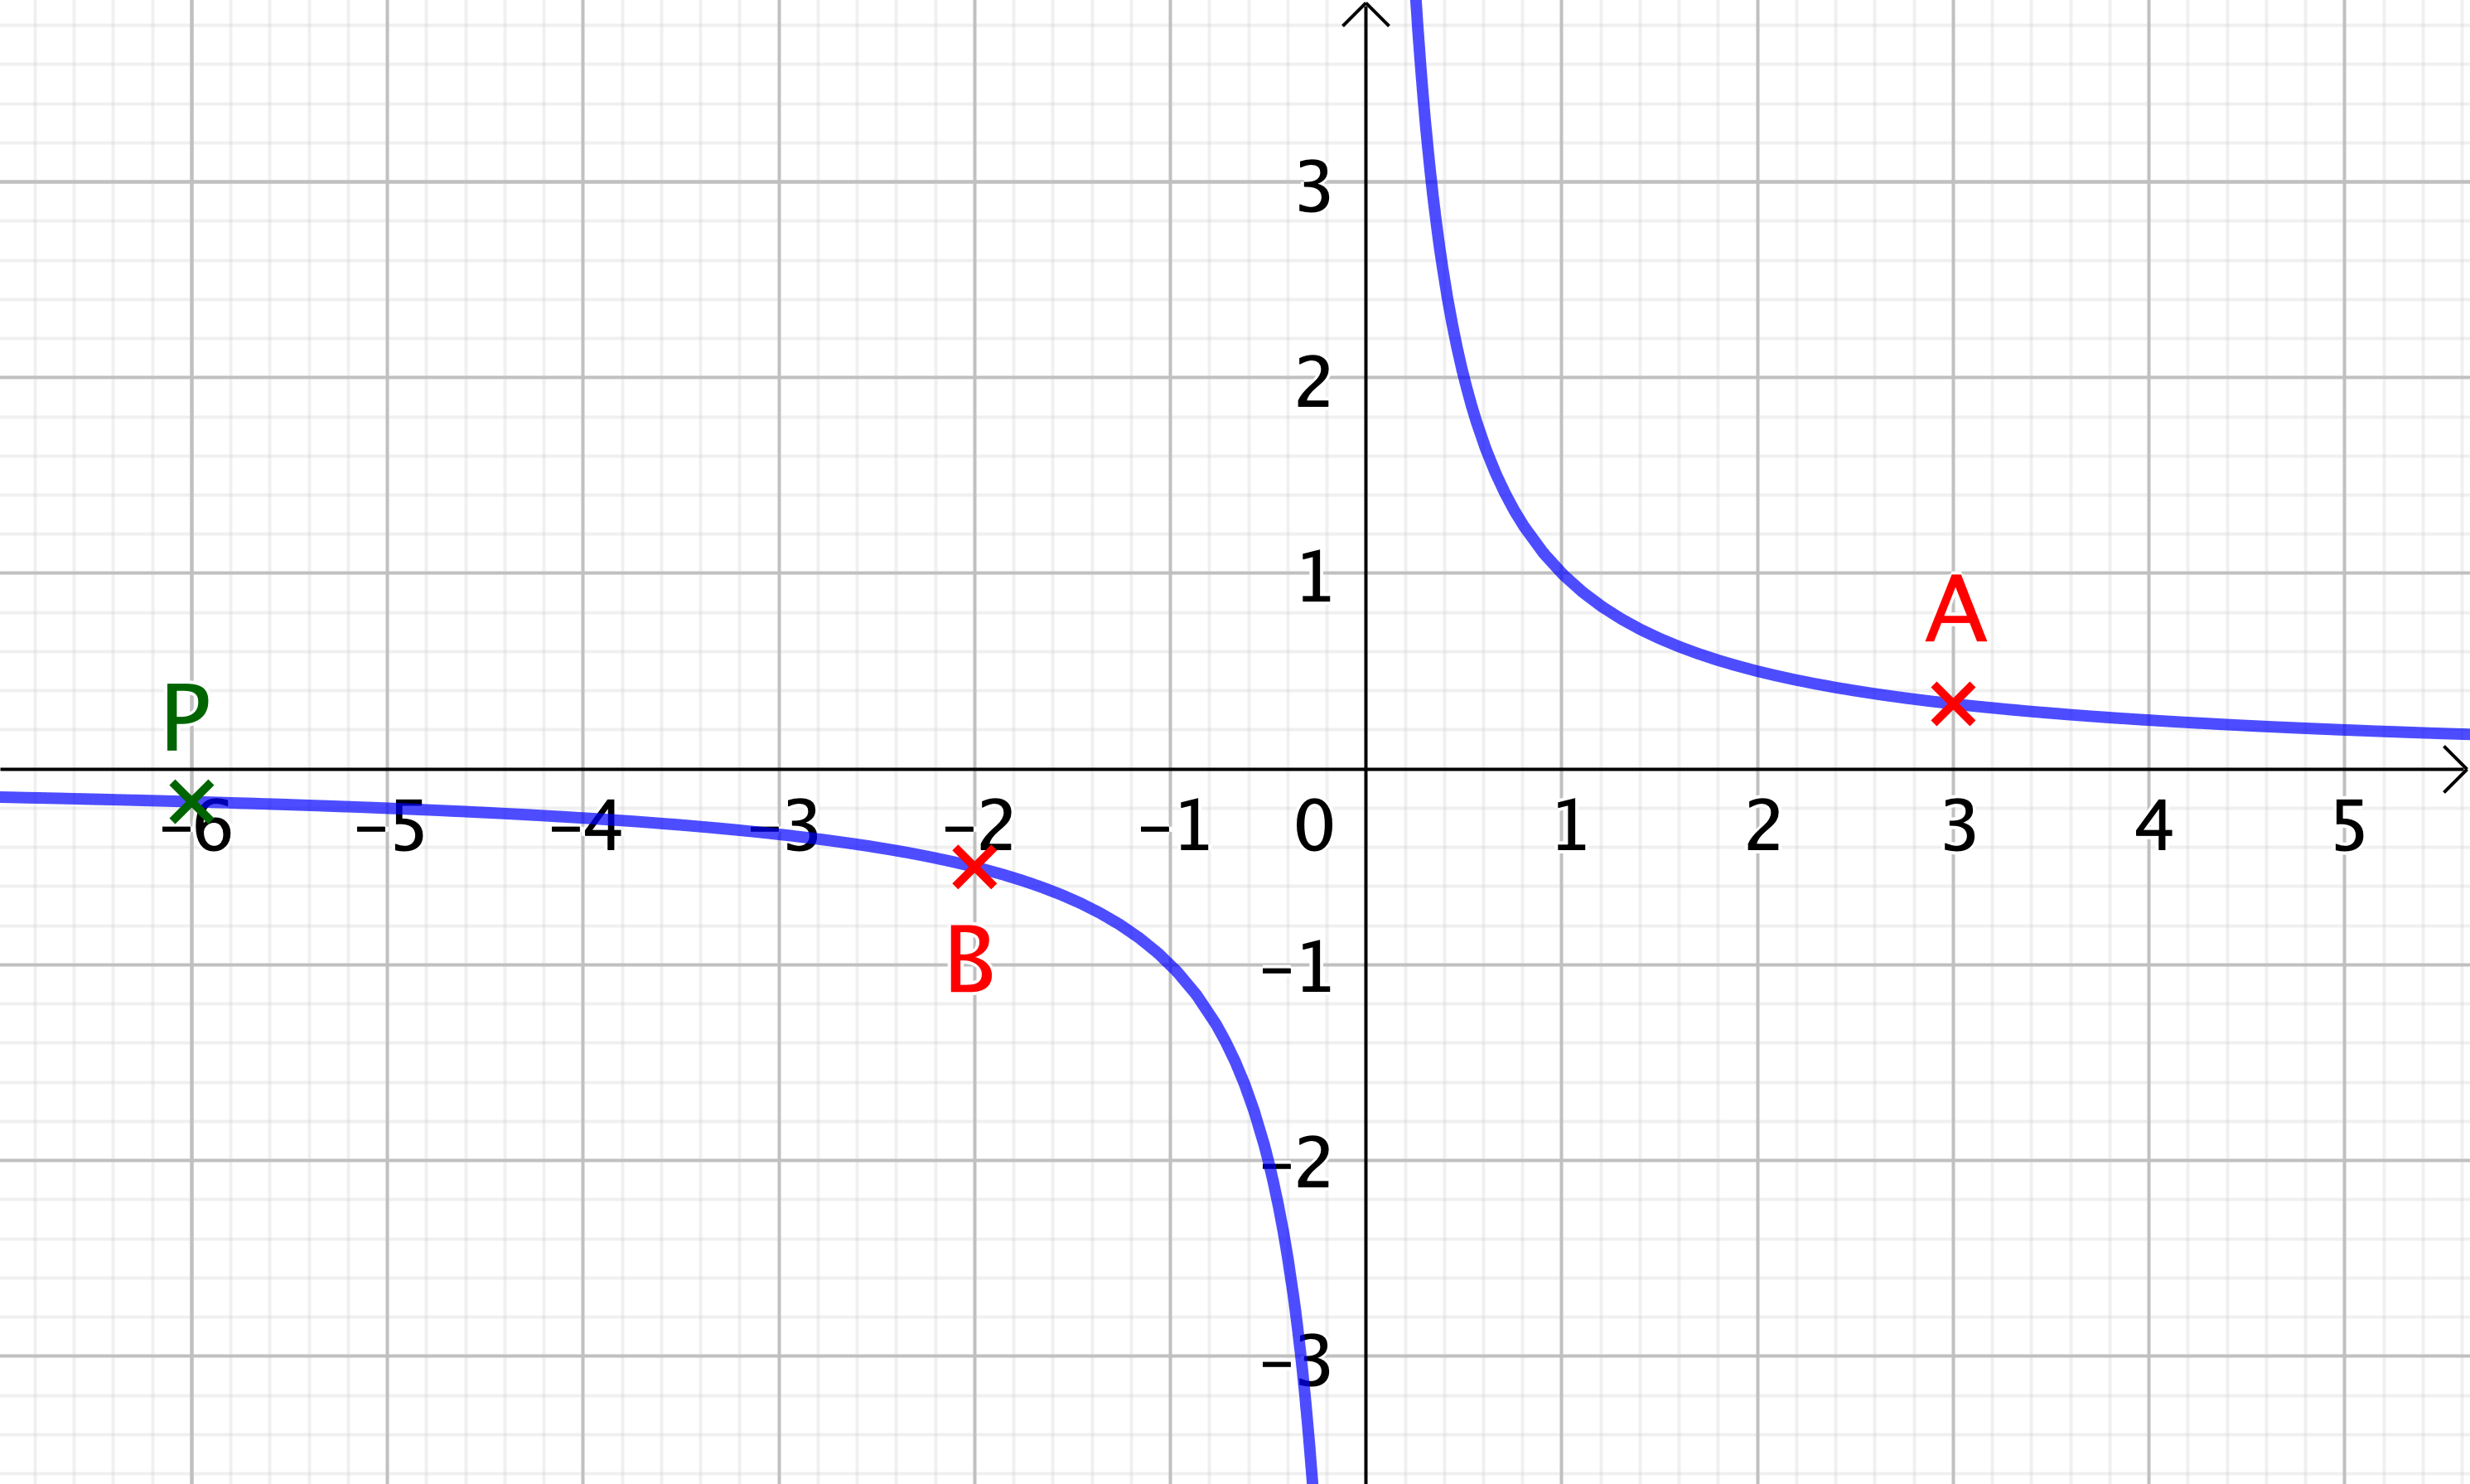
\includegraphics[scale = .8]{addition-on-parabolas/conjecture/a-and-b-diff-signs.png}}
	
	\smallskip
	Cas où $a < 0$ et $b > 0$
\end{multicols}
	
\begin{center}
	\footnotesize
	\itshape

	\fbox{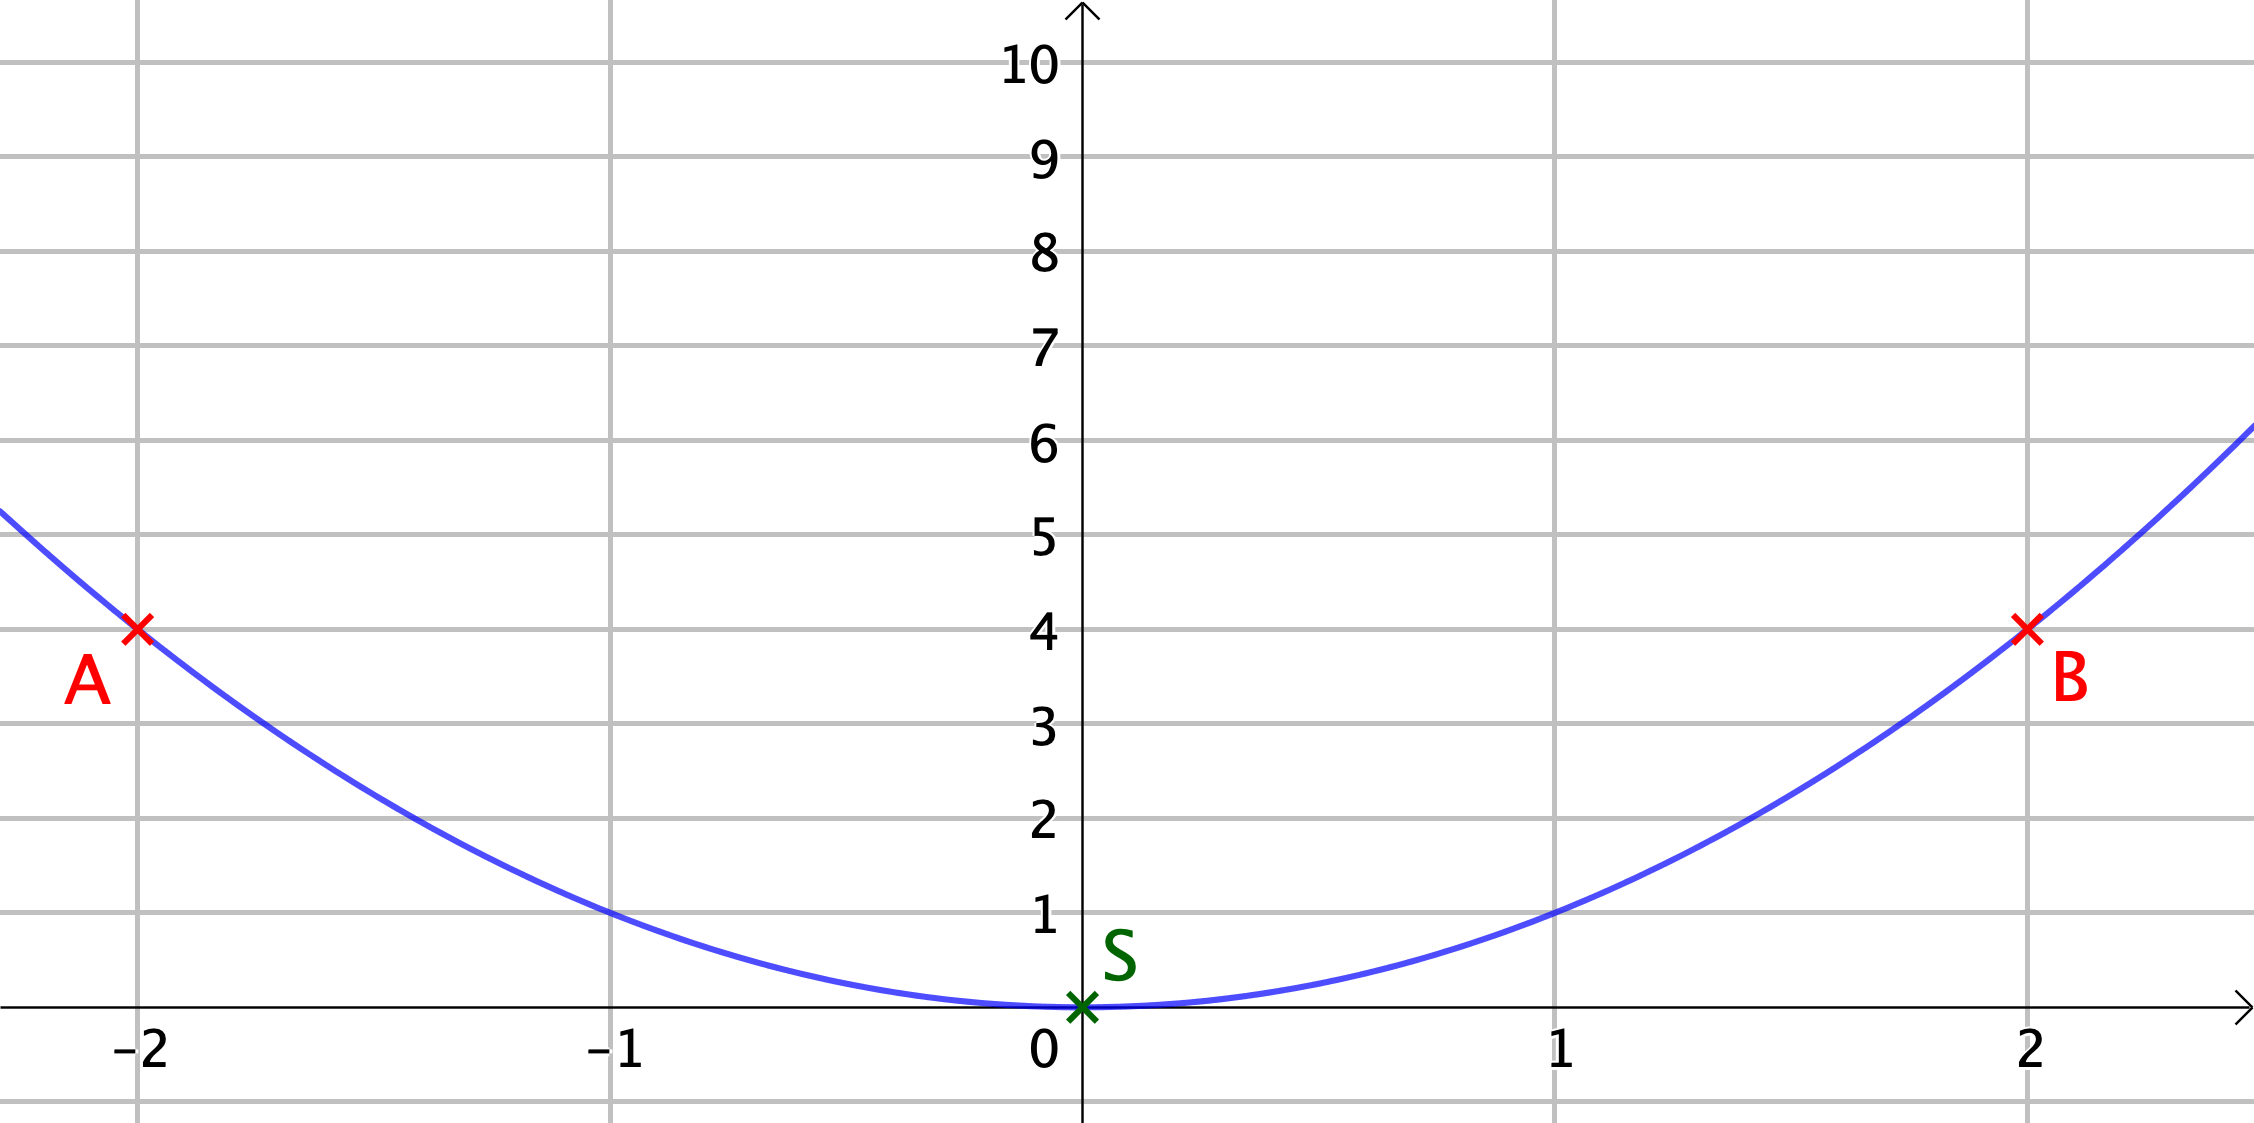
\includegraphics[scale = .8]{addition-on-parabolas/conjecture/a-and-b-opposite.png}}
	
	\smallskip
	Cas où $a = -b$
\end{center}


\newpage

Pour mieux voir ce qu'il se passe, traçons quelques droites. Voici ce que cela donne.

\begin{multicols}{2}
	\center
	\footnotesize
	\itshape

	\fbox{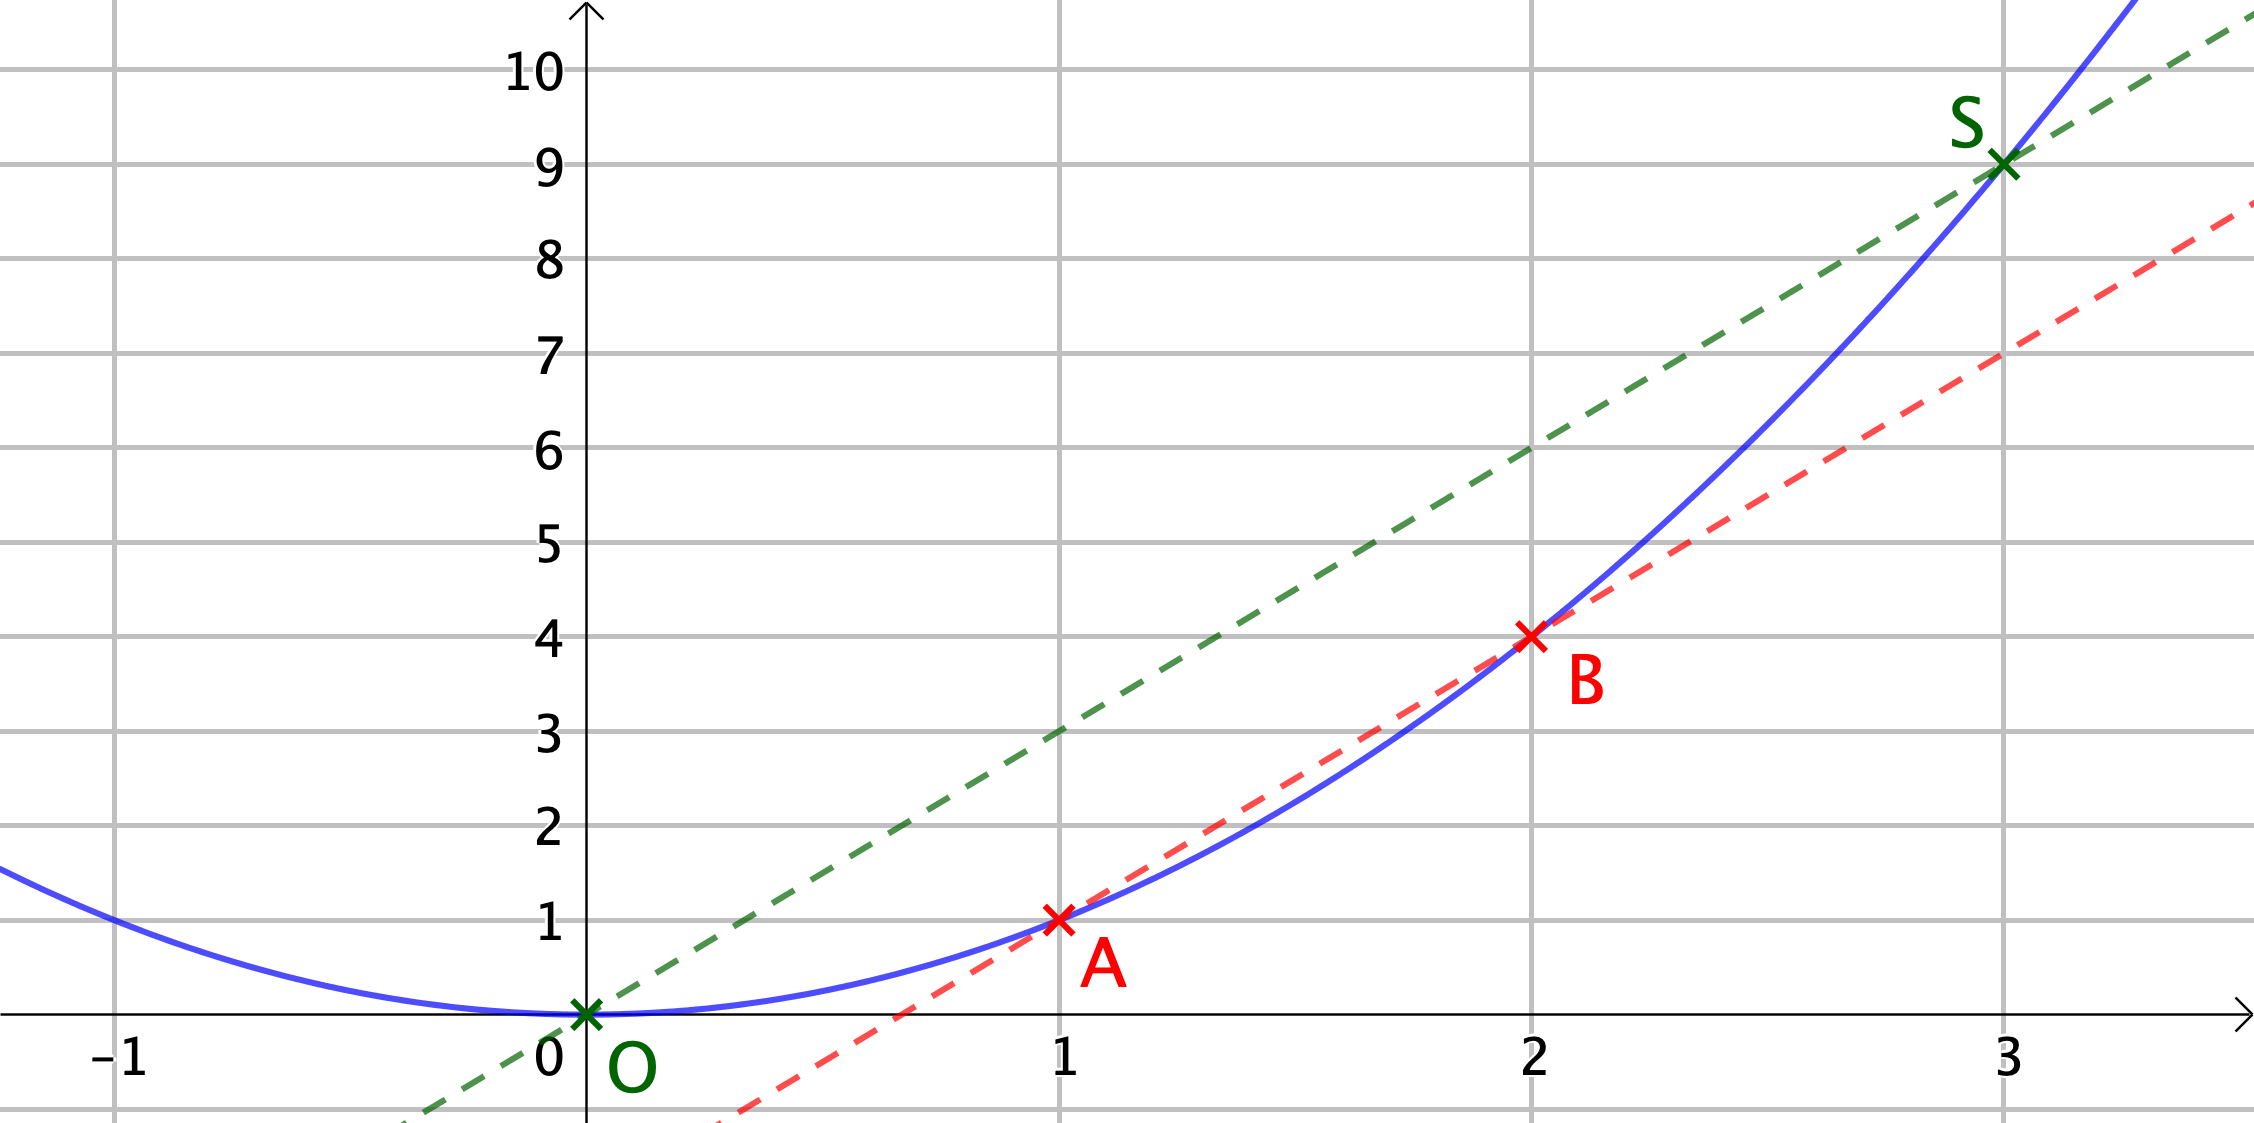
\includegraphics[scale = .8]{addition-on-parabolas/conjecture/a-and-b-positive-with-lines.png}}
	
	\smallskip
	Cas où $a > 0$ et $b > 0$

	\columnbreak
	
	\fbox{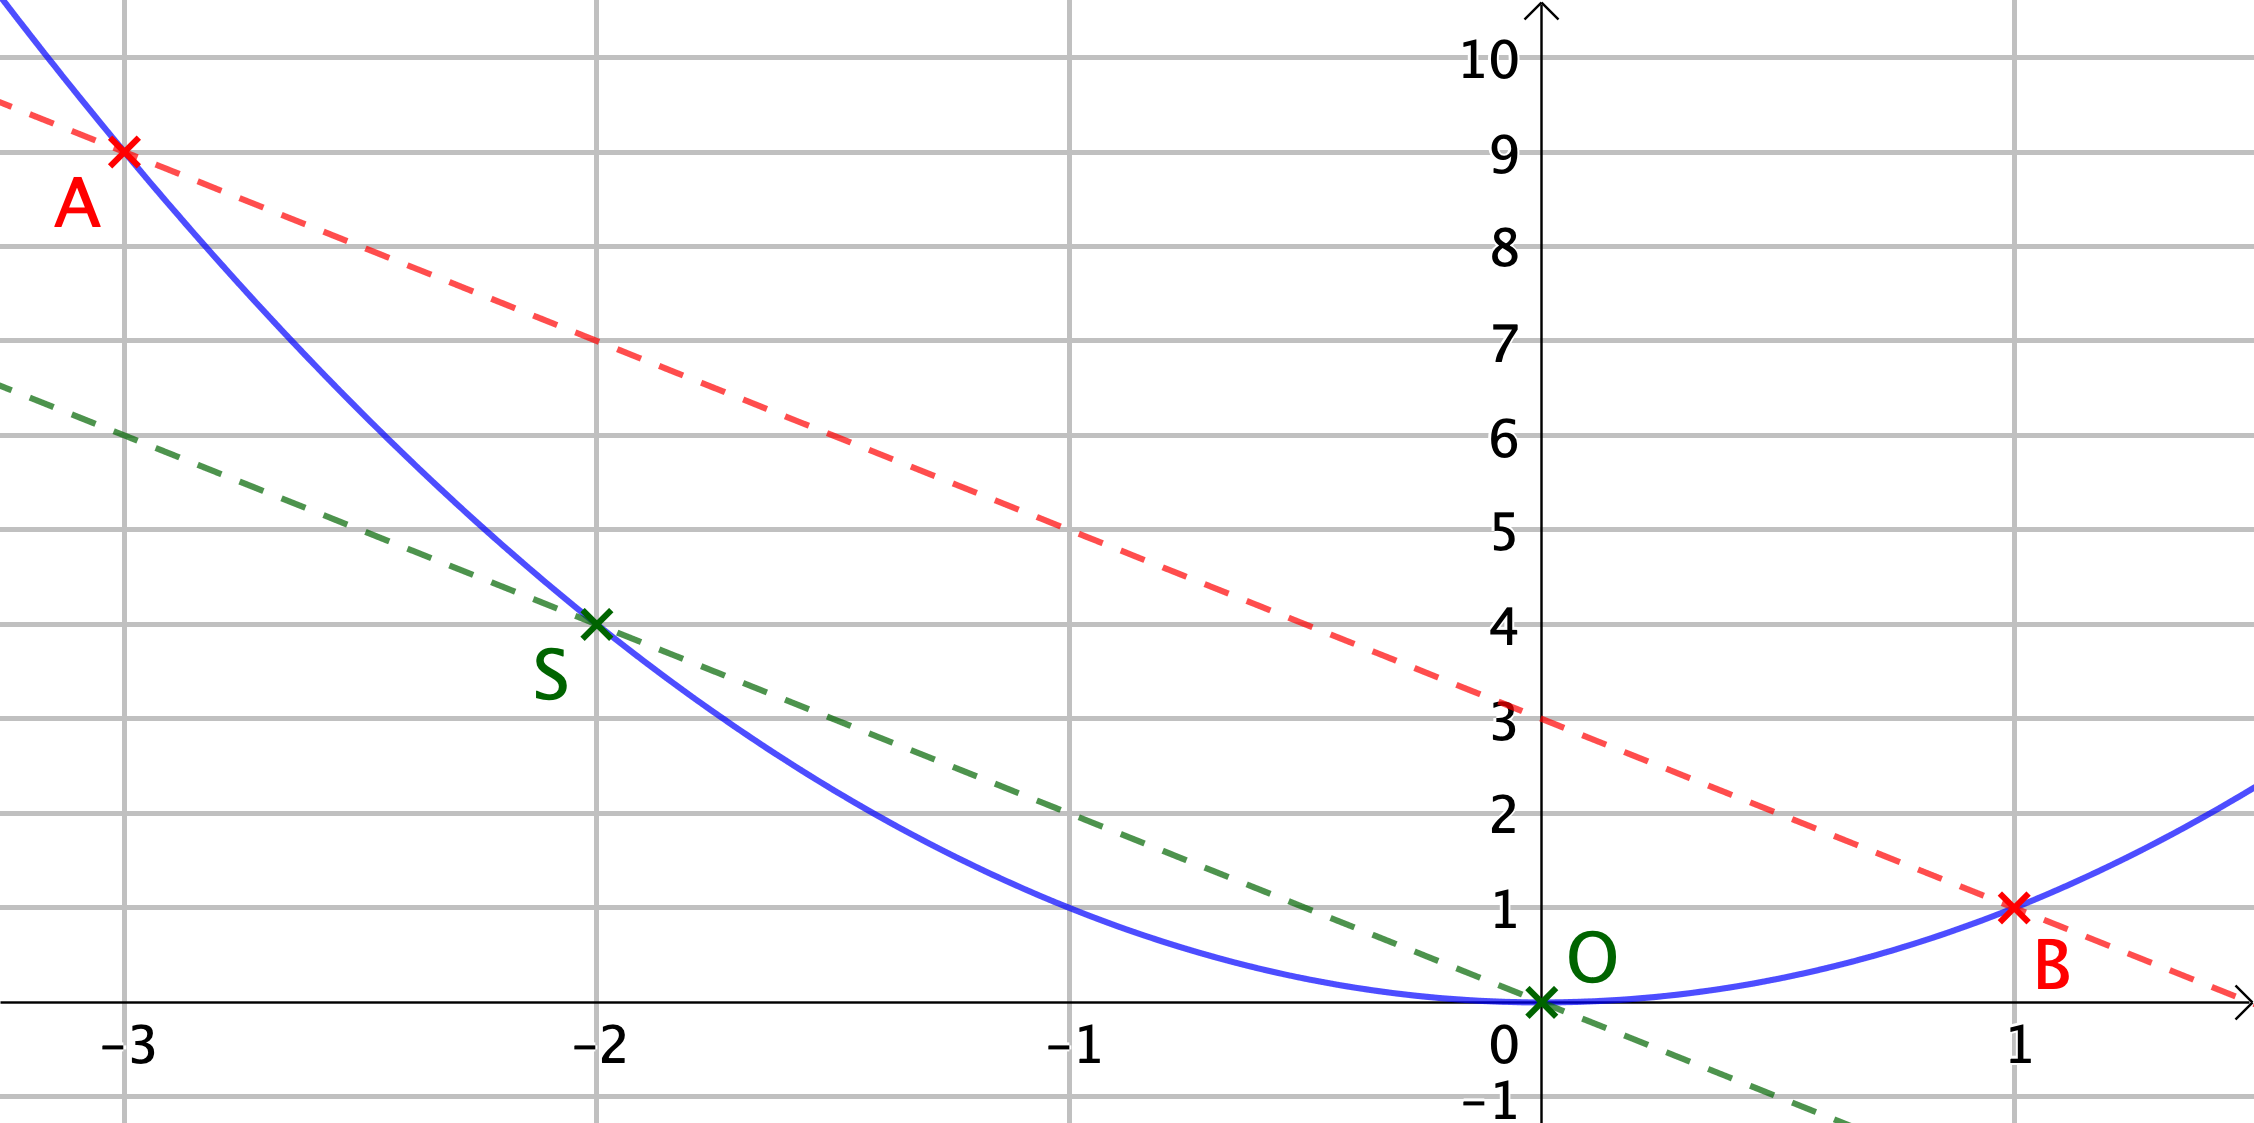
\includegraphics[scale = .8]{addition-on-parabolas/conjecture/a-and-b-diff-signs-with-lines.png}}
	
	\smallskip
	Cas où $a < 0$ et $b > 0$
\end{multicols}
	
\begin{center}
	\footnotesize
	\itshape

	\fbox{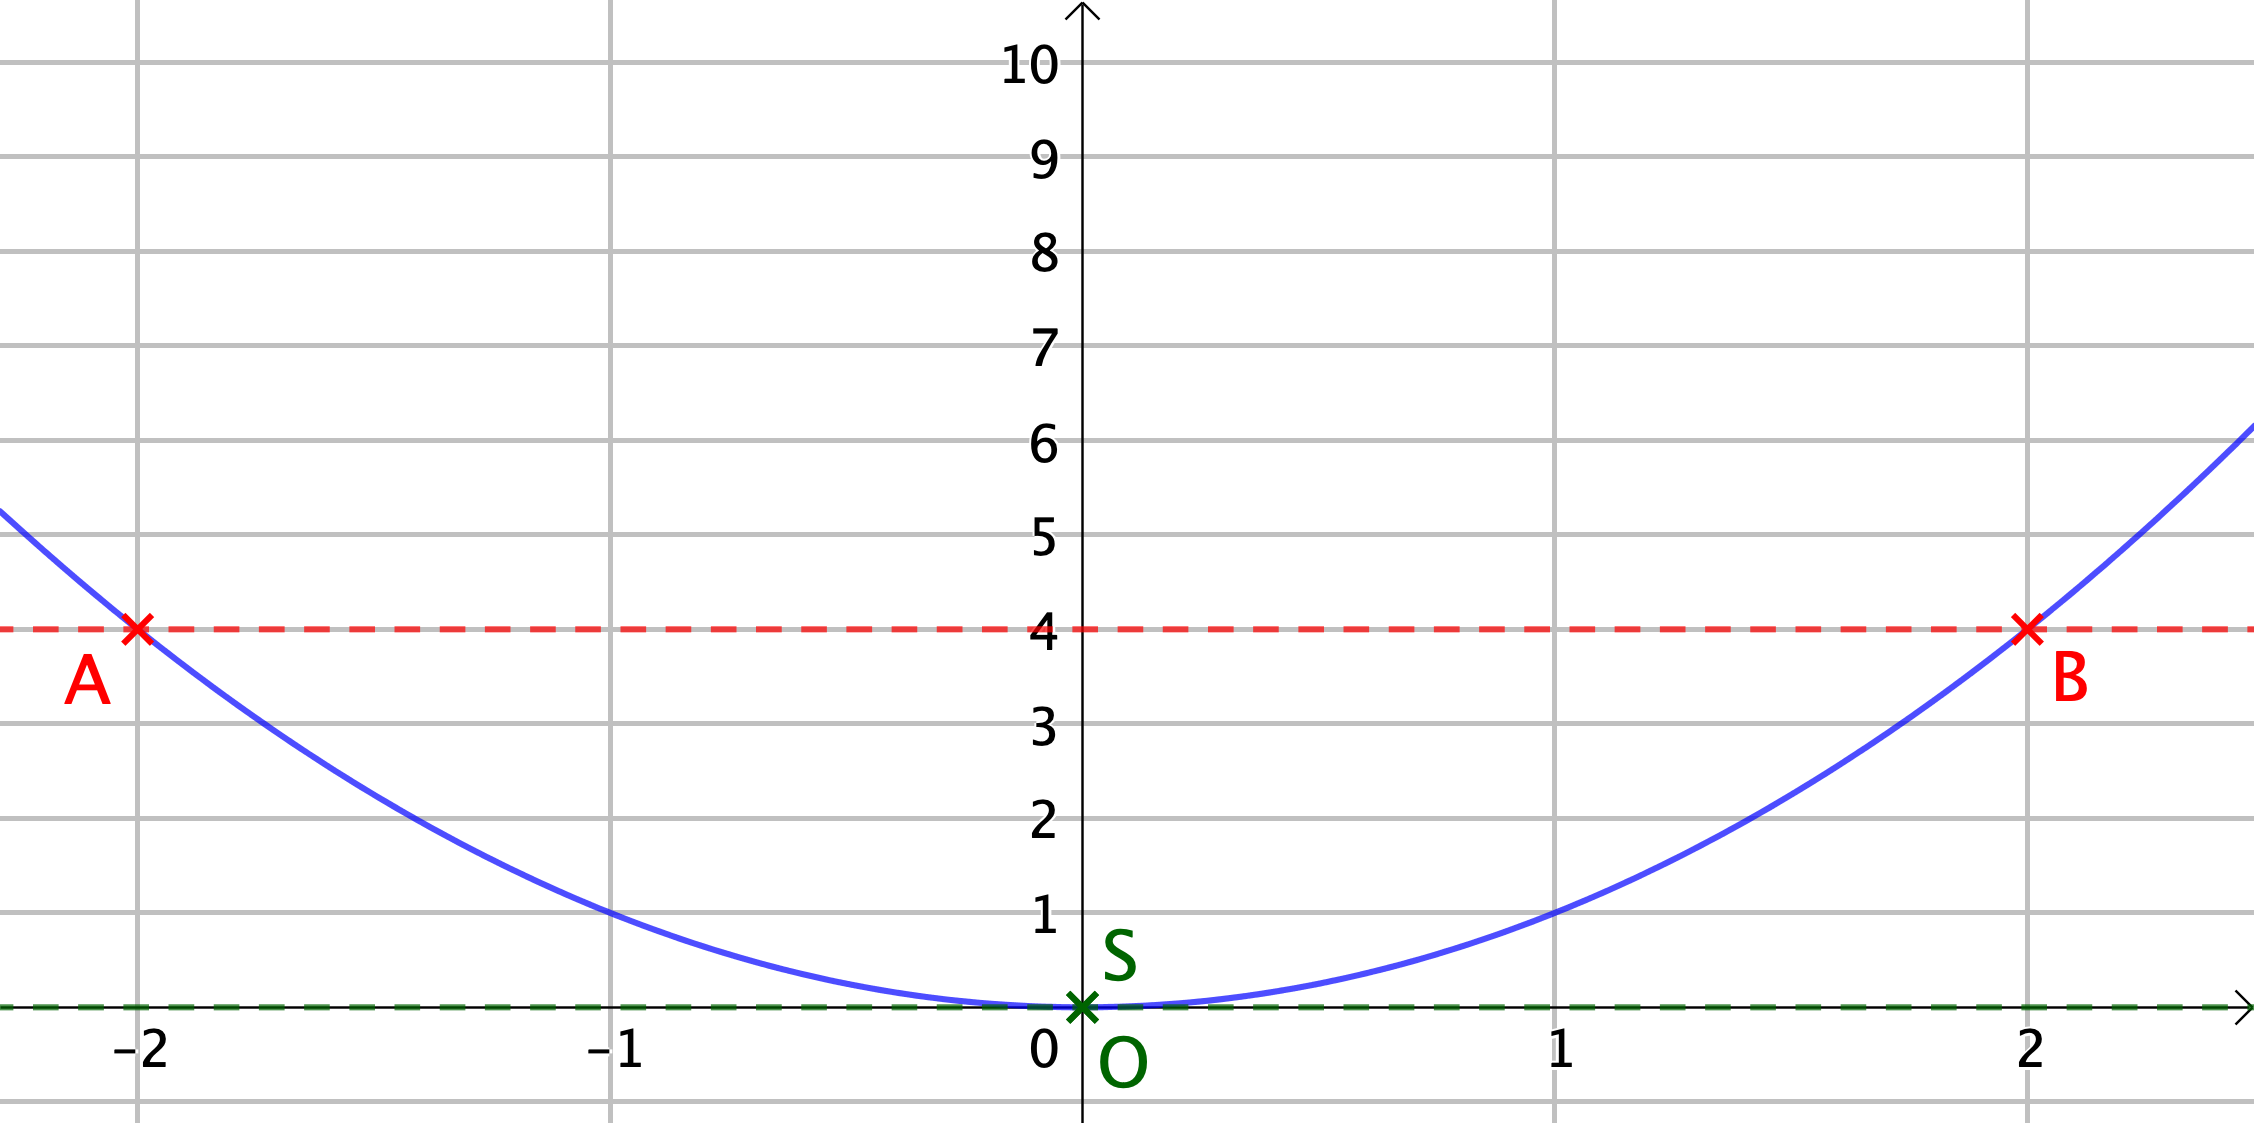
\includegraphics[scale = .8]{addition-on-parabolas/conjecture/a-and-b-opposite-with-lines.png}}
	
	\smallskip
	Cas où $a = -b$
\end{center}


\medskip

Il devient évident de conjecturer que le point $S$ se construit géométriquement comme suit.

\begin{enumerate}
	\item \label{point-1} Si $x_A \neq \pm \, x_B$ alors on construit la parallèle à $(AB)$ passant par $O$ l'origine du repère. Le point $S$ est le second point d'intersection de cette parallèle avec $\setgeo{P}$  \emph{(notons qu'une droite coupe $\setgeo{P}$ en au plus deux points)}.

	\item Si $x_A = - x_B$ alors $S = O$ . Notons au passage que l'on peut voir ceci comme un cas limite du précédent avec un point d'intersection \squote{double}.

	\item Si $x_A = x_B \neq 0$ , on procède comme au point (\ref{point-1}) mais avec la parallèle à la tangente en $A$ à la parabole $\setgeo{P}$ .
\end{enumerate}


La section qui suit va valider cette conjecture qui donne un moyen très capillotracté de calculer une somme de deux réels via la parabole $\setgeo{P}$ .
Plus sérieusement, la construction ci-dessus est une propriété géométrique très jolie de la parabole $\setgeo{P}$ .
\label{conjecture}


\section{Une preuve}\label{proof}

Revenons à nos entiers signés écrits sur $8$ bits en reprenant le calcul de $84 - 101 = -17$ tout en nous inspirant de ce qui a été vu dans la section précédente avec la base $10$.
Ici $256 = 2^8$ joue le même rôle que $1000 = 10^3$ avant. Nous avons ajouté des cases grises pour le bit du calcul intermédiaire, et nous avons indiqué les complémentations
\footnote{
	Nous utiliserons \emph{\og complémentation \fg} comme abréviation de \emph{\og complément à $2$ plus un \fg}. 
}
en mettant sur fond vert les bits les plus à gauche..

\medskip

\begin{center}
\begin{tabular}{ll}
	    & \!\!\binary{Za1010100}  	\\
	$-$ & \!\!\binary{Za1100101} 	\\[.8ex]
	\hline
	\hline 							\\[-2ex]
	    & \!\!\binary{Za1010100} 	\\
	$+$ & \!\!\binary{*a0011011} 	\\[.8ex]
	\hline \\[-2ex]
	$=$ & \!\!\binary{Uz1101111} 	\\[.8ex]
	\hline
	\hline 							\\[-2ex]
	$-$ & \!\!\binary{ca0010001} 	\\
\end{tabular}
\end{center}

\medskip

La dernière complémentation avec ajout d'un signe vient du $0$ sur fond gris et du fait qu'une seule complémentation préparatoire a été faite avant.
Tout s'éclaire !


\smallskip

Reprenons de même le cas de $84 - 61 = 23$ où l'on avait une retenue à ignorer. On fait comme précédemment.

\medskip

\begin{center}
\begin{tabular}{ll}
	    & \!\!\binary{Za1010100}  	\\
	$-$ & \!\!\binary{Za0111101} 	\\[.8ex]
	\hline
	\hline 							\\[-2ex]
	    & \!\!\binary{Za1010100} 	\\
	$+$ & \!\!\binary{*a1000011} 	\\[.8ex]
	\hline \\[-2ex]
	$=$ & \!\!\binary{Uu0010111} 	\\[.8ex]
	\hline
	\hline 							\\[-2ex]
	$+$ & \!\!\binary{Za0010111} 	\\
\end{tabular}
\end{center}

\medskip

Avec le nouvel éclairage, nous n'avons qu'à garder les bits sur fond blanc, le signe du résultat étant positif
\footnote{
	Il y a eu une seule complémentation préparatoire et le bit intermédiaire est $1$.
}.


\smallskip


Dans les deux cas précédents, au lieu de considérer un bit intermédiaire, il suffit d'effectuer directement le calcul de retenue sur le bit de gauche modulo $2$, ce calcul traduisant celui sur le nombre de complémentations préparatoires et du chiffre intermédiaire en gris dans nos deux exemples ci-dessus. On peut ainsi faire plus directement comme suit.
\begin{multicols}{2}
\begin{center}
\begin{tabular}{ll}
	    & \!\!\binary{Z1010100}  	\\
	$-$ & \!\!\binary{Z1100101} 	\\[.8ex]
	\hline
	\hline 							\\[-2ex]
	    & \!\!\binary{Z1010100} 	\\
	$+$ & \!\!\binary{*0011011} 	\\[.8ex]
	\hline \\[-2ex]
	$=$ & \!\!\binary{U1101111} 	\\[.8ex]
	\hline
	\hline 							\\[-2ex]
	$-$ & \!\!\binary{c0010001} 	\\
\end{tabular}
\end{center}

\null\vfill

\columnbreak

\begin{center}
\begin{tabular}{ll}
	    & \!\!\binary{Z1010100}  	\\
	$-$ & \!\!\binary{Z0111101} 	\\[.8ex]
	\hline
	\hline 							\\[-2ex]
	    & \!\!\binary{Z1010100} 	\\
	$+$ & \!\!\binary{*1000011} 	\\[.8ex]
	\hline \\[-2ex]
	$=$ & \!\!\binary{Z0010111} 	\\[.8ex]
	\hline
	\hline 							\\[-2ex]
	$+$ & \!\!\binary{Z0010111} 	\\
\end{tabular}
\end{center}
\end{multicols}






\smallskip

Plus généralement, avec la façon de stocker les entiers signés, nous avons alors les correspondances suivantes où les entiers additionnés $a$ et $b$ sont dans $\intervalC{-128}{127}$ et leur somme aussi, ce qui revient à ne considérer que les cas de non dépassement de capacité.
\begin{multicols}{4}
    \begin{center}
	\begin{tabular}{ll}
	    & \!\!\binary{Z-}  		\\
	$-$ & \!\!\binary{Z-} 		\\[.8ex]
	\hline
	\hline 						\\[-2ex]
	    & \!\!\binary{Z-} 		\\
	$+$ & \!\!\binary{*-} 		\\[.8ex]
	\hline \\[-2ex]
	$=$ & \!\!\binary{Z-} 	    \\
	\end{tabular}
	
	\medskip\itshape\footnotesize
	
	Soustraction 1
	
	de deux naturels
	\end{center}


	\null\vfill
	\columnbreak
	
	
	\begin{center}
	\begin{tabular}{ll}
	    & \!\!\binary{Z-}  		\\
	$-$ & \!\!\binary{Z-} 		\\[.8ex]
	\hline
	\hline 						\\[-2ex]
	    & \!\!\binary{Z-} 		\\
	$+$ & \!\!\binary{*-} 		\\[.8ex]
	\hline \\[-2ex]
	$=$ & \!\!\binary{U-} 	\\
	\end{tabular}
	
	\medskip\itshape\footnotesize
	
	Soustraction 2
	
	de deux naturels
	\end{center}


	\null\vfill
	\columnbreak
	
	
	\begin{center}
	\begin{tabular}{ll}
	$-$ & \!\!\binary{Z-}  		\\
	$-$ & \!\!\binary{Z-} 		\\[.8ex]
	\hline
	\hline 						\\[-2ex]
	    & \!\!\binary{*-} 		\\
	$+$ & \!\!\binary{*-} 		\\[.8ex]
	\hline \\[-2ex]
	$=$ & \!\!\binary{Z-} 	\\
	\end{tabular}
	
	\medskip\itshape\footnotesize
	
	Addition 1 de
	
	deux relatifs négatifs
	\end{center}


	\null\vfill
	\columnbreak
	
	
	\begin{center}
	\begin{tabular}{ll}
	$-$ & \!\!\binary{Z-}  		\\
	$-$ & \!\!\binary{Z-} 		\\[.8ex]
	\hline
	\hline 						\\[-2ex]
	    & \!\!\binary{*-} 		\\
	$+$ & \!\!\binary{*-} 		\\[.8ex]
	\hline \\[-2ex]
	$=$ & \!\!\binary{U-} 	\\
	\end{tabular}
	
	\medskip\itshape\footnotesize
	
	Addition 2 de
	
	deux relatifs négatifs
	\end{center}


	\null\vfill
\end{multicols}

\vspace{-1.5em}

Les soustractions et l'addition 2 ne posent aucun souci.
Par contre l'addition 1 est problématique avec son résultat positif. 
En fait cette addition contredit notre hypothèse de non dépassement de capacité. Nous allons voir pourquoi.

\medskip

Le cas de l'addition 1 correspond à $(a ; b) \in \intervalC{-128}{-1}^2$ tel que $(128 + a) + (128 + b) \in \intervalC{0}{127}$ soit $0 \leq 256 + a + b \leq 127$ \emph{i.e.} $-256 \leq a + b \leq -129$ ce qui correspond à un dépassement de capacité comme annoncé.
 
\medskip

Ceci achève de démontrer la validité des procédés d'addition et de soustraction d'entiers signés dans les cas de non dépassement de capacité.
Notez que le cas évident d'une addition de deux naturels a été omis, et aussi que $-a + b = b - a = b + (-a)$ et le fait qu'un changement de signe n'est autre qu'un complément à $1$ plus $1$ permettent de compléter les cas non indiqués ci-dessus.

\begin{exercise}
	Étudiez plus généralement le cas d'une base $b \in \NN_{\geq 3}$ quelconque.
\end{exercise}




\section{Coder - Étudier la \og période \fg{} d'un naturel}

Quand il ne se fige pas, le code suivant donne la \textit{\og période \fg} d'un naturel auquel on applique le procédé présenté dans la section \ref{conjecture}.

\begin{rawcode}
n     = 20181209
nmemo = n

results = []

while n not in results:
    results.append(n)
    n = sum(int(d)**2 for d in str(n))

print(f"{nmemo} a la période suivante :")
print(results[results.index(n):])

print()

before = results[:results.index(n)]

if before:
    print("Avant la 1ère période nous avons :")
    print(before)
else:
    print("On commence directement par la période.")
\end{rawcode}

\medskip

Le code précédent, où \verb+n = 20181209+, nous affiche :

\begin{rawcode}
20181209 a la période suivante :
[16, 37, 58, 89, 145, 42, 20, 4]

Avant la 1ère période nous avons :
[20181209, 155, 51, 26, 40]
\end{rawcode}


\medskip

\begin{figure}[t]
    \centering
    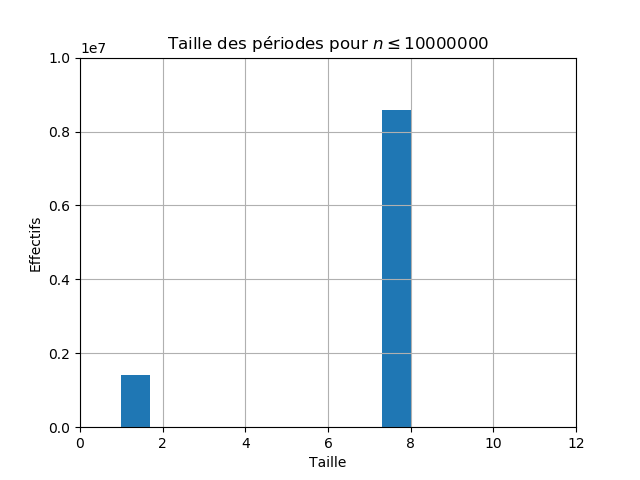
\includegraphics[scale=.9]{squares-digits/periods.png}
      \caption{Histogramme des tailles des périodes}
    \label{histogram}
\end{figure}



\medskip

Amusons-nous maintenant à représenter un histogramme des tailles des \og périodes \fg{}
À l'adresse \url{https://github.com/bc-writing/drafts}, dans le dossier \texttt{squares-digits}, vous trouverez le fichier \texttt{squareint-sizeplots.py} qui été utilisé pour obtenir le graphique
\footnote{
    À la même adresse dans le dossier \texttt{squares-digits} se trouve l'image \texttt{befores.png} qui est un histogramme des nombres de termes calculés avant l'apparition de la 1\iere{} \emph{\og période \fg{}}.
}.
Le traitement des données a été amélioré pour éviter de refaire des calculs déjà rencontrés \emph{(pour plus de précisions, se reporter aux commentaires du code)}.
Le résultat est donné dans la figure \ref{histogram} \cpageref{histogram}.



\medskip

Le graphique est frappant ! En effet, il semblerait que l'on ait soit des périodes de taille $1$, penser à $0$ et $1$, soit des périodes de taille $8$ comme pour $37 - 58 - 89 - 145 - 42 - 20 - 4 - 16$.
Magie ou coïncidence ? Les résultats de la section \ref{proof}, dont nous allons reprendre les notations, vont nous permettre de le savoir.
Tout d'abord,  d'après le fait \ref{magicmajo}, nous avons $\taille(sq(n)) < \taille(n)$ dès que $\taille(n) \geqslant 4$, donc la périodicité n'arrivera que lorsque $\taille\left( \, \sqseq{n}{k} \right) \leqslant 3$.
De plus, nous savons aussi que $\taille(sq(n)) \leqslant 3$ dès que $\taille(n) \leqslant 3$.
Tout ceci nous permet d'analyser brutalement via un programme ce qu'il se passe pour les périodes des naturels appartenant à $\ZintervalC{0}{999}$. Nous pouvons pour cela utiliser le code suivant, qui n'est absolument pas optimisé mais fait le travail immédiatement.


\newpage

\begin{rawcode}
nmax = 999

periodsfound = []

for n in range(nmax + 1):
    results = []

    while n not in results:
        results.append(n)
        n = sum(int(d)**2 for d in str(n))

    period = results[results.index(n):]

    if period not in periodsfound:
        periodsfound.append(period)

for oneperiod in periodsfound:
    print(oneperiod)
\end{rawcode}



\medskip

Le code précédent nous fournit toutes les périodes possibles.


\newpage

\begin{rawcode}
[0]
[1]
[4, 16, 37, 58, 89, 145, 42, 20]
[37, 58, 89, 145, 42, 20, 4, 16]
[89, 145, 42, 20, 4, 16, 37, 58]
[16, 37, 58, 89, 145, 42, 20, 4]
[20, 4, 16, 37, 58, 89, 145, 42]
[58, 89, 145, 42, 20, 4, 16, 37]
[42, 20, 4, 16, 37, 58, 89, 145]
[145, 42, 20, 4, 16, 37, 58, 89]
\end{rawcode}


\medskip

Et là cela devient joli car nous notons au passage que trois types de périodes :
\verb+[0]+, \verb+[1]+ et
\verb+[4, 16, 37, 58, 89, 145, 42, 20]+ avec toutes ses \emph{\og permutées circulaires \fg}.



\section{\texorpdfstring{Peut-on généraliser à un exposant $k \geqslant 3$ ?}%
                        {Peut-on généraliser à un exposant k >= 3 ?}}

Pour finir, nous allons analyser ce qu'il se passe si l'on somme à la puissance $k \geqslant 3$ au lieu d'élever au carré.
Nous reprenons des notations similaires à celles de la section \ref{proof}.
\begin{itemize}[label = \textbullet]
	\item Pour un naturel $n =  \left[ \, c_{d-1} c_{d-2} \cdots c_1 c_0 \, \right]_{10}$ avec $c_{d-1} \neq 0$,
	on pose
	$\displaystyle pw(n) = \sum_{i=0}^{d-1} (c_i)^{\,k}$
	et
	$\taille(n) = d$.
	
	\item Pour $(n \,; i) \in \NN^2$, on définit 
	$\sqseq{n}{0} = n$
	et
	$\sqseq{n}{i+1} = pw \left( \, \sqseq{n}{i} \right)$.
\end{itemize}

 

\bigskip

\begin{fact}
	$\forall n \in \NN$, $pw(n) \leqslant 9^{\,k} \, d$ où $d = \taille(n)$.
\end{fact}

\begin{proof*}
	Si $n = \left[ \, c_{d-1} c_{d-2} \cdots c_1 c_0 \, \right]_{10}$
	alors 
	$\displaystyle pw(n) = \sum_{i=0}^{d-1} (c_i)^{\,k} \leqslant \sum_{i=0}^{d-1} 9^{\,k} = 9^{\,k} \, d $.
\end{proof*}




\medskip

\begin{fact}\label{magicmajo}
	Il existe $d_0 \in \NN$ tel que $\forall n \in \NN$,	
	$[ \, \taille(n) \geqslant d_0 \Rightarrow pw(n) < n \, ]$.
\end{fact}

\begin{proof*}\label{magicmajo-proof}
	Notons $d = \taille(n)$ de sorte que $n \geqslant 10^{d-1}$.
	Compte tenu du fait précédent, nous cherchons à comparer $10^{d-1}$ et $9^{\,k} \, d$.
	
	
	\medskip
	
	Nous allons procéder de façon analogue au cas $k = 2$ démontré dans la section \ref{proof} mais en étant ici plus rigoureux dans la rédaction.
	
	
	\medskip
	
	$\exists d_0 \in \NNs$ tel que $10^{d_0 - 1} > 9^{\,k} d_0 > 9^{\,k  - 1}$ . Ceci s'obtient en utilisant la croissance comparée des fonctions $f(x) = 10^{x - 1}$ et $g(x) = 9^{\,k} x$.


	\medskip
	
	Montrons par récurrence sur $d \geqslant d_0$ que $10^{d - 1} > 9^{\,k} d$ .
	Ceci donnera $n \geqslant 10^{d - 1} > 9^{\,k} d \geqslant pow(n)$ d'où $n > pow(n)$ dès que $d \geqslant d_0$ comme souhaité.

	\begin{itemize}[label=\small\textbullet]
		\item \emph{Initialisation.}
		Par choix de $d_0$ , nous avons $10^{d-1} > 9^{\,k} d$ si $d = d_0$.

		\item \emph{Hérédité.}
		Faisons l'hypothèse que $10^{d-1} > 9^{\,k} d$ est vérifiée pour un naturel $d \geqslant d_0$ \emph{\og fixé quelconque \fg}.

		\smallskip
		
		\noindent
		Nous avons : $10^{(d+1)-1} = 10\times10^{d-1} = 10^{d-1} + 9\times10^{d-1} > 10^{d-1} + 9^{\,k}$
		en utilisant au passage $10^{d-1} \geqslant 10^{d_0-1} > 9^{\,k  - 1}$.

		\smallskip
		
		\noindent
		Comme $10^{d-1} > 9^{\,k} d$, nous avons ensuite $10^{(d+1)-1} > 9^{\,k} d + 9^{\,k} = 9^{\,k} (d+ 1)$ .
		L'inégalité est donc vérifiée au rang suivant $(d+1)$. 

		\item \emph{Conclusion.}
		Par récurrence sur $d \geqslant d_0$ , nous avons $10^{d - 1} > 9^{\,k} d$ pour tout naturel $d$ tel que $d \geqslant d_0$ .
	\end{itemize}
\end{proof*}
	

\medskip

\begin{remark}
	Informatiquement une valeur de $d_0$ peut s'obtenir en testant $10^{d - 1} > 9^{\,k} d$ successivement pour les naturels non nuls $d$.
	
	
	\medskip
	
	Pour gagner du temps, on peut tester les valeurs successives de $2^i$ pour $i = 0, 1, 2, \dots$ pour obtenir $D$ tel que $10^{D - 1} > 9^{\,k} D$ . Si la valeur de $D$ est trop grande pour faire des tests brutaux, on peut chercher la valeur minimale de $d$ tel que $10^{d - 1} > 9^{\,k} d$ en utilisant une recherche de type dichotomique. 
\end{remark}


\medskip

\begin{fact}\label{beautifulproof}
	$\forall n \in \NN$, la suite $\left( \, \sqseq{n}{i} \right)_{i \in \NN}$ est ultimement périodique.
\end{fact}

\begin{proof*}
	Tout est en fait contenu dans le fait \ref{magicmajo}, dont on reprend la signification de $d_0$. Expliquons pourquoi.
	\begin{itemize}[label = \textbullet]
		\item Le fait \ref{magicmajo} donne l'existence d'un indice $i_0 \in \NN$ tel que $\taille\left( \, \sqseq{n}{i_0} \right) < d_0$ \emph{(dans le cas contraire, on pourrait construire une suite strictement décroissante de naturels)}.

		\item Si pour tout naturel $i \in \ZintervalCO{i_0}{+\infty}$ , $\taille\left( \, \sqseq{n}{i} \right) < d_0$ , nous avons l'ultime périodicité via le principe des tiroirs \emph{(si besoin revoir la fin de la section \ref{proof})}.

		\item Sinon il existe $i\,^\prime_0 \in \ZintervalO{i_0}{+\infty}$ tel que $\taille\left( \, \sqseq{n}{i\,^\prime_0} \right) \geqslant d_0$. Comme dans le premier point, nous pouvons alors trouver $i_1 \in \ZintervalO{i\,^\prime_0}{+\infty}$ tel que $\taille\left( \, \sqseq{n}{i_1} \right) < d_0$.
		
		\item En répétant notre raisonnement,
		on peut aboutir à une situation similaire au 2\ieme{} point, et c'est gagné. 
		
		\noindent
		Sinon on arrive à construire une suite strictement croissante $\left( i_k \right)_k$ d'indices tels que $\forall k \in \NN$, $\taille\left( \, \sqseq{n}{i_k} \right) < d_0$. Le principe des tiroirs s'applique ici aussi !
	\end{itemize}
\end{proof*}



\medskip

\begin{remark}
	La preuve précédente montre que pour rechercher toutes les périodes il \emph{\og suffit \fg} d'étudier les naturels appartenant à $\ZintervalCO{0}{10^{d_0}}$ .
\end{remark}





\bigskip

\hrule

\section{AFFAIRE À SUIVRE...}

\bigskip

\hrule


%\section{Quelles périodes déterminées informatiquement}
%
%
{\Huge ????} La preuve du fait \ref{beautifulproof} permet de justifier que le programme suivant, pour peu qu'il ne se fige pas, fournit toutes les périodes possibles pour un exposant $p \geqslant 3$ connu.


n = 3
\begin{rawcode}
[0]
[1]
[55, 250, 133]
[136, 244]
[153]
[160, 217, 352]
[370]
[371]
[407]
[919, 1459]
\end{rawcode}


n = 4
\begin{rawcode}
[0]
[1]
[1138, 4179, 9219, 13139, 6725, 4338, 4514]
[1634]
[2178, 6514]
[8208]
[9474]
\end{rawcode}


n = 5
\begin{rawcode}

\end{rawcode}



\end{document}
